% Kapitel 2 - Related Work / Literaturanalyse
\section{System Introduction}\label{sec:RelatedWork}

The previous chapter aimed at shedding light on the process of testing in the modern automotive industry and the problems faced as a result. It is important to understand the systems being dealt with before setting any fixed goals. It is a crucial pre-requisite for setting goals as the adaptation and corresponding fine tuning would be a direct by-product of this. This section introduces the existing approach and methods to tackle the aforementioned problem of enormous data size. 
%-------------------------------------------------------------------------------------------------------------------------------------------------------------

\subsection{Introduction to Hardware} \label{sec:hardware}
 As mentioned earlier on, this thesis deals with Life Time Tester systems for Environmental Qualifications. The life cycles of the test specimens are simulated and the are simulated and thus the behaviour over the service life is determined. Various properties such as current or voltage can be monitored. Furthermore, it is possible, for example, to combine the test facility with a climate chamber for testing temperature cycles. 

Testing is carried out within the framework of a Qualification Program (\textbf{QP}) according to certain specifications. Generally speaking, there are two basic work packages that fall under the heading of testing. The first is the so-called Design Verification (\textbf{DV}). This generally includes all theoretical processes that are intended to ensure that all design requirements for the product are fulfilled. The DV is followed by the so-called product validation (PV). Here, the functionality of the product including the requirements is tested in practical test procedures. In the context of a \textbf{QP}(Qualification Program), one also speaks of a so-called DV/PV. Many hardware components for controlling the inputs for the data acquisition devices are interconnected, the most important of which are explained here. 

The basic framework for the test system is a 19-inch test rack in which all components are integrated. A photo of the front view of the test system can be seen in \hyperref[fig:Testrack]{Figure 2}. The test rack has a height of approx. 1.50 m, on which the test PC stands, and it is divided into individual height units (HE) according to the rack standard. The test units can be tested with the standard bus systems CAN (FD), LIN, Ethernet and Flexray. A total of eight \gls{DUT}s can be connected to the test rack at the same time. can be connected to the test rack at the same time. They are connected to the test system via 108-pole Harting industrial connectors. These are fully assigned and, depending on the project configuration, a different number of data lines and bus systems are required. In total, the following data bus communications are possible :

\begin{itemize}
    \item 7 x CAN
    \item 4 x LIN
    \item 9 x Ethernet
    \item 4 x Flexray
\end{itemize}

\begin{figure}
  \centering
  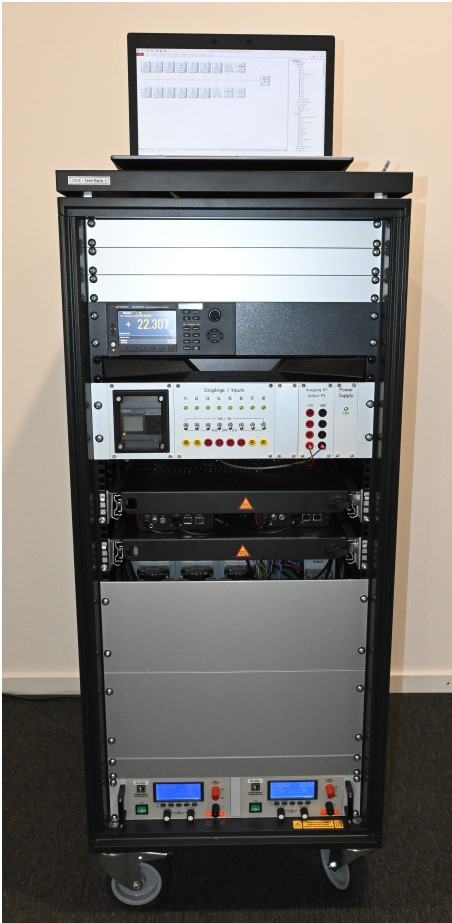
\includegraphics[width= 0.6\textwidth]{images/Testrack.jpg}
  \caption{19 inch "wide" Testrack}
  \label{fig:Testrack}
\end{figure}

In addition, individual measuring channels for the voltage and current measurements of the DUTs are integrated, for example. The supply voltages for Kl. 15 (switched positive from ignition lock) and Kl.30 (positive line from battery) according to DIN 72552 can be modelled including the necessary ground (GND) lines. 

One signal LED per DUT is integrated for each connected terminal. There is a power supply unit at the bottom of the Testrack which feeds in the DC voltage for all the DUTs. \begin{comment}
The power supply units are PSI 5000A DC Laboratory Power Supply from Elektro-Automatik [12], which is shown at the bottom of Figure 2.2. Figure 2.2 at the bottom.
\end{comment}
In addition, the front panel contains the connection for a PT-1000 temperature sensor, which is responsible for measuring an external chamber temperature, and a connection for an external trigger. The central measuring unit of the test system is the Keysight Data Acquisition System. This is integrated into the front of the test rack. It can be seen in \hyperref[fig:Testrack]{Figure 2} in the upper part with the current temperature display. Three different measuring cards, which are connected to the test rack via 50-pin Sub-D plugs to the test rack, enable measurements of different amplitudes/sizes.

The current is measured for each DUT via a shunt resistor R\textsubscript{s}. The voltage drop U\textsubscript{s} at the shunt is measured via a measuring line and the corresponding current is calculated according to Ohm's law (see equation 2.1), the corresponding current is calculated.

\begin{equation}
I_s= \frac{U_s}{R_s}\
\end{equation}

The individual DUTs are switched via automotive relays. If the relay is closed, a voltage drop can be measured at the shunt resistor and the corresponding current at the DUT can be calculated via equation 2.1. Two low-power LEDs (for terminal 15 and terminal 30) indicate to the operator whether a DUT is connected. The hardware equipment for controlling the data buses in the form of frame, load and error generation comes from Vector Informatik GmbH. The following network interfaces are included in each test system in a 19 inch rack system:
\begin{itemize}
    \item 4 x VN640 ( CAN, LIN, FlexRay)
    \item 2 x VN5620 (Ethernet, CAN)
    \item 1 x VN1630 A (CAN, LIN)
\end{itemize}

All Vector hardware is usually integrated horizontally in the lower drawer system shown in \hyperref[fig:Testrack]{Figure 2}. The individual data sheets of the Vector hardware are available on the manufacturer's homepage. The connection to the test computer is made via a serial USB interface. For this purpose, another pull-out height unit is equipped with USB hubs for communication of the Vector control units with the test computer. For each Vector control unit, the individual channels can be individually configured in the so-called \emph{Vector-Hardware-Configuration}.

A portable test computer is available for each of the four test systems. The development and test software CANoe from Vector Informatik and further test automation software are essential for carrying out the tests. 

%Riener \cite{riener} hat sich die Frage gestellt, was sich aus dem Einsatz von Autopilotensystemen in der Luftfahrt für den Bereich des (teil)automatisierten Fahrens in der Automobilindustrie übertragen/lernen lässt und was man für die Gestaltung der Interaktion übertragbar machen könnte. usw. usw.
%Gold et al. thematisierten die Frage, ``zu welchem Zeitpunkt, vor dem Auftreten einer Systemgrenze, muss das FAS die Aufmerksamkeit des Fahrers auf sich ziehen, um eine erfolgreiche Übernahme durch den Fahrer auch dann sicherzustellen, wenn er sich nicht im Loop befindet.'' \cite{gold} %
Hierzu wurde eine Studie mit 32 Probanden in einem High-Fidelity-Fahrsimulator bei BMW durchgeführt. Das Szenario beschreibt eine Fahrt mit 120 km/h auf einer dreispurigen Autobahn, bei der das vorausfahrende Auto einen Unfall verursacht und somit den Fahrer zu handeln zwingt. 17 Probanden haben dieses Szenario als Referenz manuell durchfahren, wobei der Unfall zum Einen fünf Sekunden, zum Anderen 7 Sekunden entfernt war. Die gleichen Zeiten wurden für die Probanden der hochautomatisierten Zeit eingehalten um die Übergabe einzuleiten.  

Folgende Ergebnisse konnten aus dieser Studie gezogen werden:
\begin{itemize}
	\item[1.] Die geringe Zeit bis zur Übernahme lässt die Probanden schneller zu einer Entscheidung und Reaktion kommen, dennoch ist deren Qualität schlecht.
	\item[2.] Mit der sich verringernden Zeit bis zur Übernahme nehmen die Kontrollblicke in Spiegel und über die Schulter ab, hingegen nimmt die Beschleunigung zu, sowie auch das Betätigen der Bremse.
	\item[3.] Vergleicht man die Probanden aus der Referenzfahrt und der hochautomatisierten Fahrt, wird deutlich, dass bei den Probanden der hochautomatisierten Fahrt bis zu dreimal so hohe Beschleunigungen erzielt wurden. Auch werden hier viele plötzliche Bremsmanöver durchgeführt. 
\end{itemize}

Die Studie belegt unter diesen experimentellen Bedingungen, dass bei vollständiger Ablenkung des Fahrers bei hochautomatisierter Fahrt noch bei sieben Sekunden Übernahmezeit ein Automatisierungseffekt auftritt. Das bedeutet, dass der Fahrer durch die fahr-fremde Nebentätigkeit stark abgelenkt ist und der automatisierten Fahrt vertraut. Dies führt zu solchen Reaktionen bei unerwarteter Bekanntmachung von Übernahmen. 







\newpage

\subsection{Introduction to Software}

The basis for the environmental qualification tests is laid in Vector CANoe by means of a configuration (.cfg-file). It allows to analyse a multi-bus communication of ECUs or entire systems.
CANoe performs following functions \cite{pd} : 
\begin{itemize}
    \item Creation of simulation models which simulate the behavior of the ECUs
    \item Graphic and text based analysis windows are provided for evaluating the results
    \item Create custom interfaces to control the simulation and tests or to display the analysis data
    \item Ease of programming through the CAN Access Programming Language (CAPL) to support simulation, analysis and testing
\end{itemize}

In the measurement setup, the data flow for the individual bus communications is graphically displayed and configured. The typical measurement setup of a CANoe configuration can be found below. In the measurement setup, so-called CAPL program nodes can be inserted, which are represented by the individual grey boxes. 


\begin{figure}[H]
	\centering
	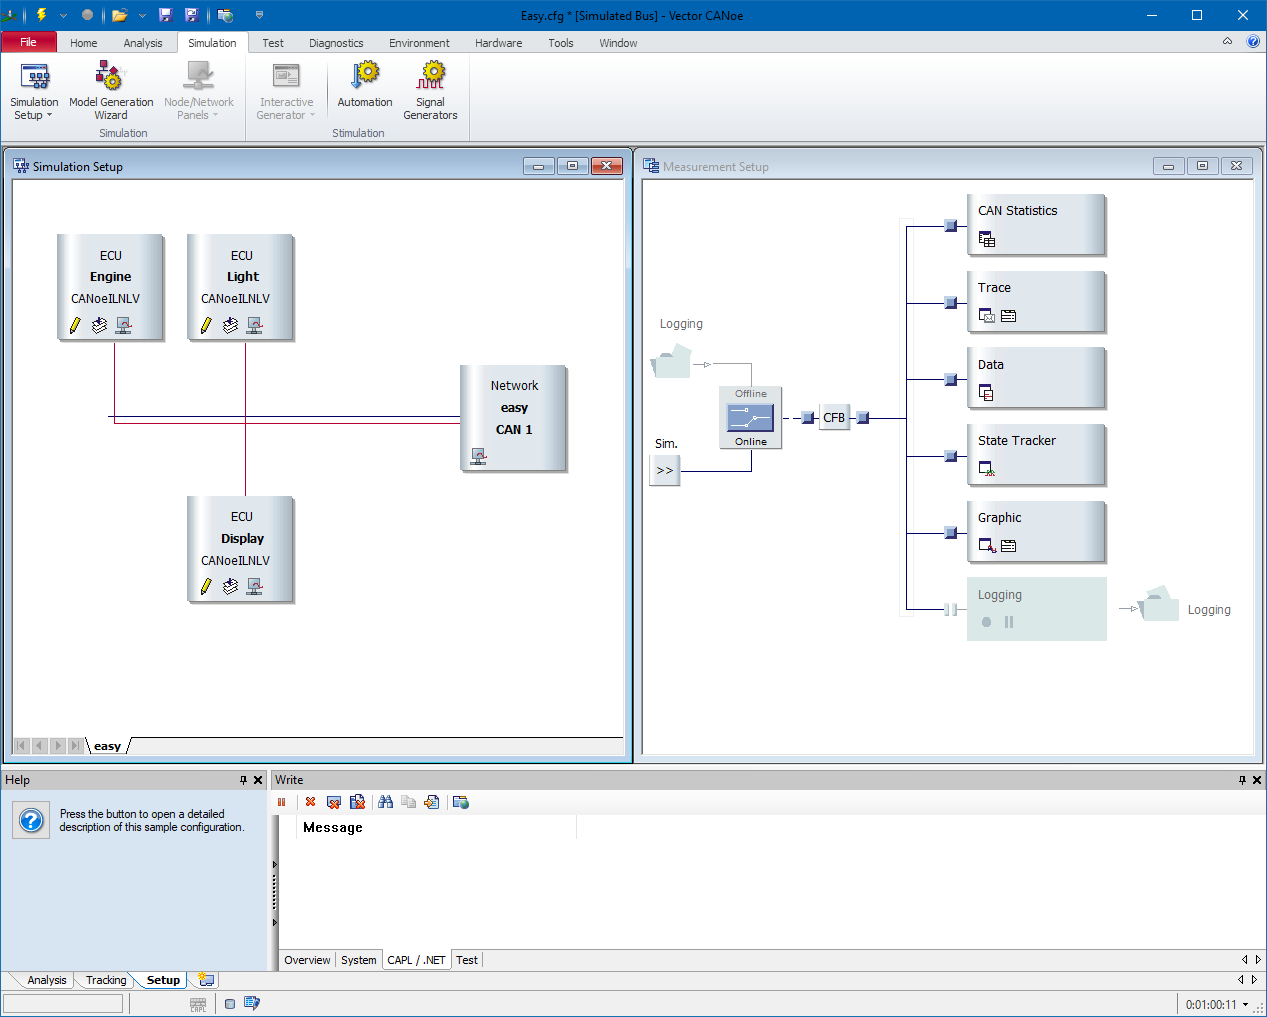
\includegraphics[width= 0.9\textwidth]{images/CANoe_Simulation_setup.png}
	\caption[CANoe Simulation and Measurement Setup]{CANoe Measurement Setup \cite{CANOE} } 
	\label{fig:Measurement Setup}
\end{figure}

Furthermore, analysis windows can be inserted with which the data can be displayed in different ways (e.g. as a graphic display of signal curves or as a display of signal values). In the so-called trace window, bus activities such as the sending of messages or error frames are listed. Individual signal values can be displayed for each message. At a later point in the work, the so-called logging of the data also plays a major role. With the logging block, bus traffic can be recorded in BLF and ASCII formats. Another feature of CANoe are user-denominated panels adapted to the test case. With the help of these, interfaces can be created for different areas of application. Panels are also used, for example, to control the simulation and test environment or to display analysis data from CAPL programs.

The automation of the test sequences is taken over by the software, which is responsible for sequencing the test cases. The time sequence of the individual tests is concretely defined via this. Some of these functions include:

\begin{itemize}
    \item Initialisation of Hardware
    \item Setting Operational Modes
    \item Begin/End of Simulation/Logging Process
    \item Set Power Supply levels
\end{itemize}

An example of this is shown in below figure for a thermal test. The 1st column in the diagram shows the individual steps, which are processed from top to bottom. Access to the test automation software system is indicated by "sys" (2nd Column). Furthermore, the 3rd column shows the command and, if applicable, the corresponding parameters in 4th column. For example, in step 10 the voltage of both power supplies is set to 12 volts. Now that a rough overview of the software components has been given, let's have a look at continuous monitoring which is an essential part of Endurance Testing. 

\begin{figure}[H]
	\centering
	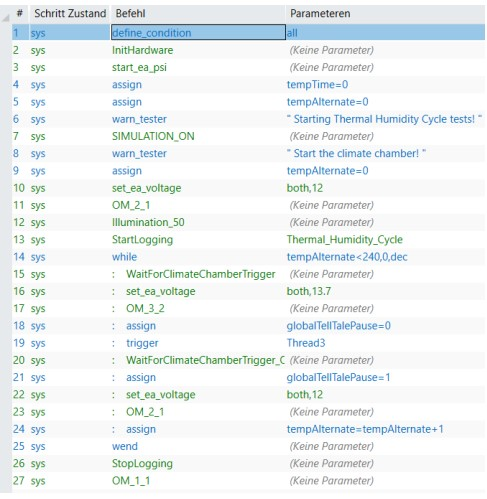
\includegraphics[width= 1\textwidth]{images/CANoe variable system.jpg}
	\caption{CANoe commands list }  
	\label{fig:CANoe commands list}
\end{figure}
\newpage
\subsubsection{Data-logging \& Storage Issues} \label{datalog}

At this point, it is important to introduce the testing procedure enabled by the software setup here called continuous monitoring. 

It is important to be able to provide the customer with measurement records that are uninterrupted over time. When testing DUTs on the basis of functional tests, logging protocols must therefore be used to prove that the assembly behaves according to specification. The keyword here is continuous monitoring. There is no clear definition of this term. If a certain frequency for logging data is specified by the customer, a more detailed analysis of this topic is not necessary, and one can work according to concrete specifications. However, direct numerical specifications for the storage interval of measurement data are often not made in customer specifications. In the following some problems are listed, for which continuous test monitoring can help \cite{ctm}.

\begin{itemize}
    \item Undetected change in environmental conditions
    \item Memory leakage
    \item Intermittent errors due to marginal test designs
    \item Performance degradation due to long-term testing
\end{itemize}

Consequently, in addition to a high measurement frequency to capture the data at all, the logging frequency is also significant. Logging is the automatic creation of a log of software processes. The frequency of logging is a directly related to the type of test and it's definition. For a test that takes only a few minutes, this frequency can be kept high and, for example, a data record can be recorded every second. The memory requirement is then kept within limits. If it is a long-running test with a duration of several hundred hours with unchanging environmental conditions, a successive reduction of the logging frequency is possible. At this point it should be noted that the diagnosis of possible errors and measurement deviations has top priority and an error control function must be ensured during a test. If a limit violation occurs, it must be possible to return to the original logging frequency.


An example of an environmental test with a large total test duration is the High Temperature Operating Endurance (HTOE) test. These tests are defined in CES's internal test definition documents known as QPP or Qualification Program Plan. The QPP is derived from various automotive test specific standards and regulations along with customer requirements. The HTOE test simulates failure modes and the cumulative damage that results from bias operation at different temperatures such as solder plastic creep, crack propagation in many materials, drying of electrolytic capacitors etc. \cite{qpp}. The temperature profile of the HTOE test as a function of time is shown in \hyperref[fig:HTOE Test Cycle]{Fig.5}. 

\begin{figure}[H]
	\centering
	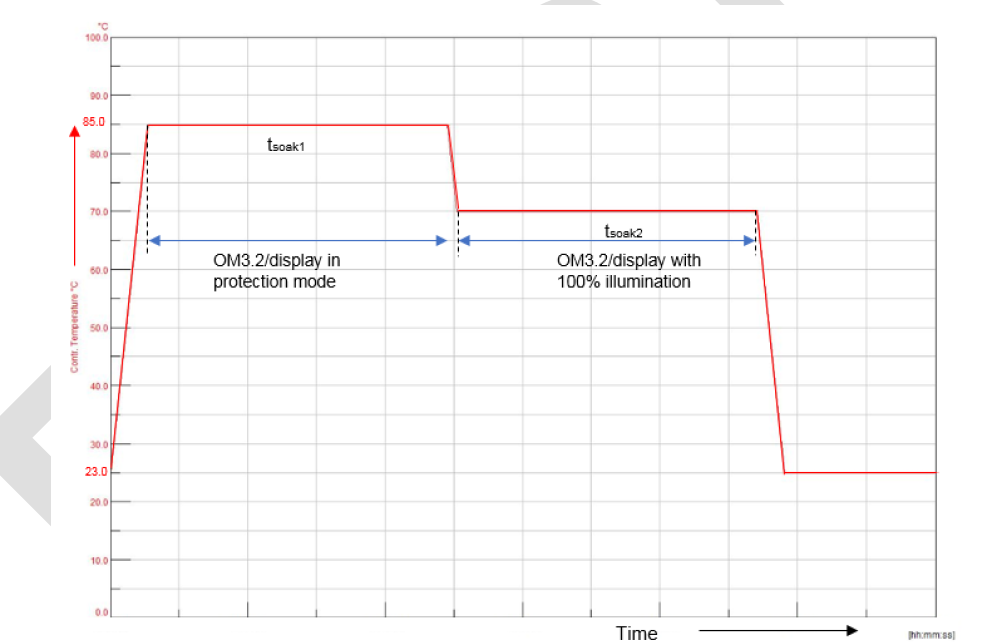
\includegraphics[width= 0.77\textwidth]{images/HTOE.png}
	\caption{HTOE}  
	\label{fig:HTOE Test Cycle}
\end{figure}

Here, for example, longer test times occur where the temperature does not change, such as in the first period when testing at 85° C. This temperature is a test standard and is defined in the AEC (Automotive Electronic Council) Q100 Qualification program for electronic components such as integrated circuits (ICs). The 85° C results from Grade Three of the Ambient Operating Temperature Range, which is defined from -40 to 85° C \cite{aec}. The test is conducted for over 850 hours. If the logging frequency is set at for example, 2 s, we would obtain ~1.5 million data points according to equation below 


\begin{equation}
Datapoints = \frac{Hours * 3600}{Sample Frequency}
\end{equation}

Depending on how the format of logging block is setup in CANoe shown in \hyperref[fig:Measurement Setup]{Figure 3}, each data point could be above 200-250 bytes. This is shown in image below as 'length':

\begin{figure}[H]
	\centering
	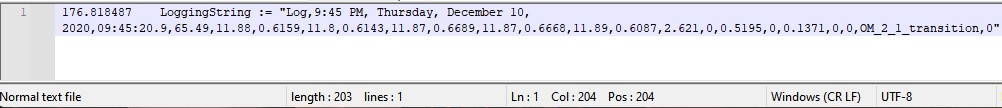
\includegraphics[width= 0.9\textwidth]{images/Datapoint.jpg}
	\caption{Datapoint Size }  
	\label{fig:Datapoint Size}
\end{figure}
 

\begin{equation}
Data Size (in MB ) = \frac{Datapoints * length}{1.048.576}
\end{equation}

So according to the equation above, size of total log from HTOE tests would be around 300-400 MB. There are different types of tests like HTOE defined in QPPs per Qualification round. This would mean that the penultimate size of all data log files per Qualification Test Round would be in multiple Gigabytes. Apart from the data log files shown in fig 2., the CANoe logging setup also generates ".blf" datalogging files. These files are usually in 100s of GB as shown below:

\begin{figure}[h]
  \centering
  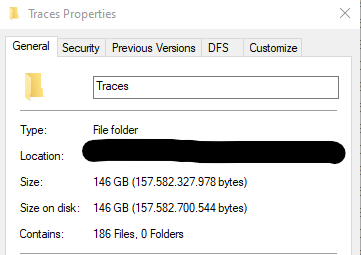
\includegraphics[width= 0.6\textwidth]{images/BLFlocationsize.png}
  \caption{.blf folder}
  \label{fig:Blf File folder}
\end{figure}


\begin{figure}[!h]
  \centering
  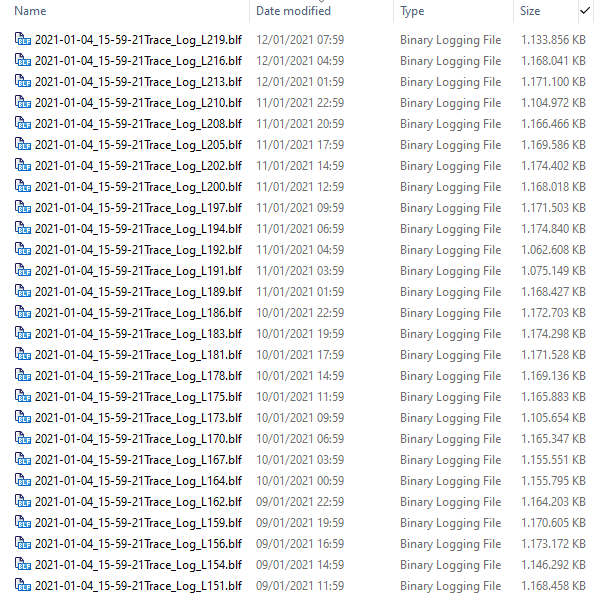
\includegraphics[width= 0.6\textwidth]{images/blfsize.png}
  \caption{.blf file sizes}
  \label{fig:Individual File Size .blf}
\end{figure}

CANoe and CANalyzer support two types of logging formats: message-based and signal-based.
\begin{itemize}
    \item Message-based - 
        A message-based format will store the traffic of bus systems and additional information about the bus communication. In general all bus events (messages) will be logged together with other information like statistics or even disturbances of the bus traffic. These logging files can be easily used for offline analyze of network traffic or for replay on the bus with CANoe.  
    \item Signal-based -
        A signal-based format will store signal values that were extracted from messages transferred over the network. All information about the message itself and additional information about the network and communication will be lost. To log a signal-based file a description (database) for decoding the signal values has to be provided. Signal-based files cannot be directly replayed on the bus but can be easily used for signal analyze in CANoe, CANape or third party tools.
\end{itemize}

ASCII Logging Files (.asc)

\begin{itemize}
    \item Message-based format for reading and writing
    \item Standard ASCII representation
    \item Used for data exchange with third-party programs or to include trace data in documents
    \item Supports messages of all bus systems, system variables, environment variables, internal events, markers and comments
\end{itemize}

Note: ASCII is not recommended at high data rates due to its poorer performance. BLF and MDF format are much better suited for this.

BLF Logging File (.blf) - A .blf file is a binary logging format file created by Vector Informatik CANoe or CANalyzer. It contains a record of the events routed through a car's controller area network (CAN). CANoe and CANalyzer users can review the events a .blf file contains or replay the events on a CAN.


\begin{itemize}
    \item Message-based format for reading and writing
    \item Binary Logging Format (binary format)
    \item Stores the data in binary format in a very efficient way in terms of file size and read/write performance
    \item Supports messages of all bus systems, system variables, environment variables, internal events, markers, and comments
\end{itemize}

BLF is recommended for all new logging \cite{blf}. Hence, all the default logging occurs on CANoe by means of a .blf file which are huge in size. The type of logging file can be set via Logging block in the measurement setup of CANoe described earlier. This thesis will study methods to reduce file size of both log-file types. 

The existing state of implementation of data logging process involves down sampling the logging rate. Down-sampling refers to the process of reducing the number of samples in a digital signal, typically for the purpose of reducing the amount of data that needs to be processed or stored. This can be done by discarding some of the samples, or by averaging multiple samples together. In image processing, down-sampling refers to the process of reducing the number of pixels in an image. This can be done by discarding some of the pixels, or by averaging the values of multiple pixels together. The goal of down-sampling is usually to reduce the computational and storage requirements of an image processing pipeline, while still preserving the important information in the image. According to existing setting, the user can configure the sampling rate before testrun using a GUI created using CANoe \& CAPL. This is demonstrated below : 

\begin{figure}[h]
  \centering
  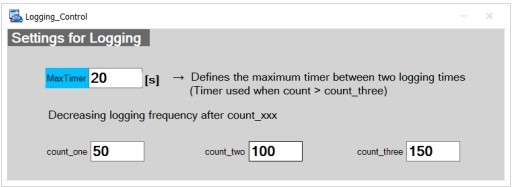
\includegraphics[width= 0.6\textwidth]{images/loggingfreq.jpg}
  \caption{Down-sampling}
  \label{fig:downsampling}
\end{figure}

Upon test setup, using this GUI the user can set the sampling rate. The "Max. Timer" option is used for setting the maximum period of data logging. However, before Max. Timer is implemented the logging process undergoes 3 step calculation, i.e, "count\_one", "count\_two", "count\_three". Initially data logging occurs at a frequency set by the Logging block mentioned earlier. The count steps are counter based flags established to check for invalid data during that particular increment period. Invalid data is determined by values that are outside the tolerance ranges defined for the test. As shown in figure, during increment, data will be monitored based on default data log frequency until 50 counts, if no error occurs till 50 counts, the average value of 50 data points is logged into the system. Thereafter counter is incremented to count\_two and then similarly after 100 non error increments, the averaged value of 100 data points is logged and then similarly for count\_three. If count\_three also provides error free data monitoring, then the data logging period is set to 20 s. Thereafter, the 
data logged is an average of values in the period of Max. Timer. The averaging is also influenced by a counter defined pre-test run "AvgNoofMeas". Towards, the end a reduced data log file is generated that is substantially down-sampled yet large in size. The thesis is focused on finding a possible alternative to this approach with primary focus on achieving maximum compression without loss of data. 
%-------------------------------------------------------------------------------------------------------------------------------------------------------------
\begin{comment}
\subsection{Research direction 2} \label{sec:rw_dir2}
\cite{wintersberger} befasst sich mit einer umfassenden und klar definierten Taxonomie der zwei Hautprozesse ``handover'' und ``handback''. Er kommt zu folgender Schlussfolgerung:

\begin{itemize}
	\item[1.] Handover - von der automatisierten zur manuellen Fahrt			  
	\item[2.] Handback - von der manuellen zur automatisierten Fahrt			  
\end{itemize}


\subsubsection{Relevanz für die eigene Arbeit - Direction 2}

Lorem ipsum Lorem ipsum.


\subsection{Schlussfolgerung}
Zusammenfassung des Kapitels, Ableitung von Empfehlungen, etc. für die eigene Arbeit.

\begin{itemize}
	\item Lorem ipsum \autoref{sec:hardware}.
	\item Lorem ipsum lorum ipsum \autoref{sec:hardware}.
	\item Lorem ipsum \autoref{sec:rw_dir2}.
	\item ...
	\item Lorem ipsum lorem ipsum lorem ipsum\autoref{sec:rw_dir2}.
\end{itemize}
\end{comment}